\chapter{Préliminaires sur les volumes finis et le langage Python}

\noindent Ce chapitre est dédié à de brefs rappels sur l'analyse numérique par la méthode des volumes finis et quelques exemples de problèmes traités en langage Python. On détaillera les outils et quelques fonctions utiles pour assembler les différents opérateurs rencontrés dans la suite du mémoire. On commence par quelques éléments de théorie largement connus avant de passer à quelques subtilités liées au langage Python et aux librairies disponibles pour ce langage et spécialisées en calcul scientifique. Le lecteur souhaitant utiliser les éléments de codes proposés ici devra s'assurer de disposer des packages \textbf{Matplotlib}, \textbf{Numpy} ainsi que \textbf{Scipy}. Ce chapitre est largement inspiré de \cite{eymard:hal-02100732}.

\section{Exemple introductif}

On utilise un problème de Poisson en 1.D pour se familiariser avec le calcul numérique en Python. Pour les résultats d'existence, d'unicité et de régularité de la solution du problème continu, on pourra consulter par exemple \cite{brezis1983}. 

L'analyse du schéma obtenu par la méthode des volumes finis sur un maillage admissible est donné dans l'introduction et développé dans le chapitre 5 de \cite{eymard:hal-02100732}. On trouve en particulier un argument pour l'existence ainsi que l'unicité d'une solution au problème discret, une définition de l'erreur de consistance locale dans le cadre des volumes finis, où il est question de la consistance des flux - voire la comparaison, dans le même ouvrage, avec la notion de consistance au sens des différences finies puis d'une méthode mixte d'éléments finis. Enfin, est étudiée la convergence en norme pour une solution $\mathcal{C}^{2}$.

\subsection*{Un problème elliptique en une dimension} Soit à résoudre numériquement le problème de Dirichlet suivant
 
On considère le problème de Poisson en une dimension. On pose $\Omega := (0,1)$ et
\begin{equation*}
\left\{\begin{array}{rl}
    u''(x) & = e^x \hspace{15pt} \forall x \in \Omega \\
    u(0) & = 1 \\
    u(1) & = e
\end{array}
\right.
\end{equation*}
L'unique solution de ce problème est $u : x \mapsto e^x$. On introduit le maillage $\mathcal{T}$ de pas à l'intérieur $\Delta x$ constant égal à $1/n_x$ où $n_x$ désigne le nombre de volumes considérés. On introduit deux points aux bords, dont la valeur est donnée par les conditions de Dirichlet. Le Laplacien se discrétise en chaque point intérieur au domaine $\Omega$. Soit $K$ un volume élémentaire, alors

\begin{align*}
    \int_K \Delta u(x) dx & = \int_{\partial \Omega} (\nabla u \cdot \mathbf{n})(\gamma(s)) d\gamma(s) \\
                          & = \sum_{\sigma \in \mathcal{E}_K} F_{K,\sigma}
\end{align*}

Dans le cas $1.D$, cette somme est réduite à deux termes $$ \sum_{\sigma \in \mathcal{E}_K} F_{K,\sigma} = F_{K, +} - F_{K, -} $$ Parmi les très nombreux choix imaginables pour approcher les flux, un exemple est le choix d'une différence finie centrée $$ F_{K|L, \sigma} \sim \frac{U_{K} - U_{L}}{\Delta x} $$ Le second membre demande un nouveau choix : comment approcher la valeur de $f$ au sein du volume $K$ ? A nouveau, existent énormément de manières de procéder et un choix courant est d'utiliser la valeur moyenne de $f$ sur $K$. Une fois fixé, cela conduit à l'approximation $$ \int_K f(x) dx \sim \Delta x f_K $$ où $f_K$ est l'approximation choisie. 

On a donc un schéma discret à l'intérieur, à deux subtilités près : on remarque que lorsque $K$ est le premier (respectivement le dernier) volume de la discrétisation, l'approximation du flux fait intervenir des points fictifs : $U_{-1/2}$ ou $U_{n_x+1/2}$. On utilise alors l'extrapolation linéaire sur la face $0$, ou $n_x$ :
\begin{align*}
    & \frac{U_{1/2} + U_{-1/2}}{2} = 1 \Longleftrightarrow U_{-1/2} = 2 - U_{1/2} \\
    & \frac{U_{n_x+1/2} + U_{n_x-1/2}}{2} = e \Longleftrightarrow U_{n_x+1/2} = 2e - U_{n_x-1/2}
\end{align*}
Et on substitue ces formules dans l'expression des flux, ce qui modifie le second membre et un facteur devant un noeud existant. On obtient donc

\begin{align*}
    U_0 & = 1 \\
    \frac{U_{i+3/2} - 2 U_{i+1/2} + U_{i-1/2}}{\Delta x} & = \Delta x f_i \hspace{15pt} \forall i \in \llbracket 1, n_x \rrbracket \\
    U_{n_x+1} & = e
\end{align*}

Une implémentation Python possible pour ce problème est la suivante.
\begin{minted}{python}
from matplotlib import pyplot
import numpy

u_func = lambda x: numpy.exp(x)
f_func = lambda x: numpy.exp(x)
x0 = 0.
x1 = 1.
nx_ = numpy.array([4, 8, 16, 32, 64, 128, 256, 512, 1024, 2048, 4096])
dx_ = numpy.empty(nx_.shape[0])
err = numpy.empty(nx_.shape[0])

for l, nx in enumerate(nx_):
    dx = (x1 - x0)/ nx
    dx_[l] = dx
    x_f = numpy.linspace(x0, x1, nx+1)
    x_c = numpy.linspace(x0+dx/2, x1-dx/2, nx)
    x_ = numpy.concatenate([[x0], x_c, [x1]], axis=0)
    u = numpy.concatenate([[u_func(x0)], u_func(x_c), [u_func(x1)]], axis=0)
    
    U = numpy.zeros((nx+2))
    b = f_func(x_c)
    A = -2/dx**2 * numpy.eye(nx) + 1/dx**2 * numpy.diag(numpy.ones(nx-1), 1) + \
        1/dx**2 * numpy.diag(numpy.ones(nx-1), -1)
    # Conditions de Dirichlet
    A[0, 0] -= 1/dx**2
    b[0] -= 2*u_func(x0)/dx**2
    A[-1, -1] -= 1/dx**2
    b[-1] -= 2*u_func(x1)/dx**2
    
    # Résolution
    U[1:-1] = numpy.linalg.solve(A, b)
    U[0]    = u_func(x0)
    U[-1]   = u_func(x1)
    
    # Estimation de la norme L^2
    err[l] = numpy.sqrt(dx) * numpy.linalg.norm(U-u, ord=2)
    
pyplot.figure()
pyplot.plot(x_, U, label=r"$(U_i)$", marker='x')
pyplot.plot(x_, u, label=r"$u(x)$")
pyplot.legend()
pyplot.suptitle("Graphe de la solution.")
pyplot.show()

pyplot.figure()
pyplot.loglog(nx_, err, label="Erreur", marker="x")
pyplot.loglog(nx_, dx_, "r--", label=r"$y = dx$")
pyplot.loglog(nx_, dx_**2, "g--", label=r"$y = dx^2$")
pyplot.legend()
pyplot.show()
\end{minted}
laquelle rend les deux graphes
\begin{figure}[htp]
    \centering
    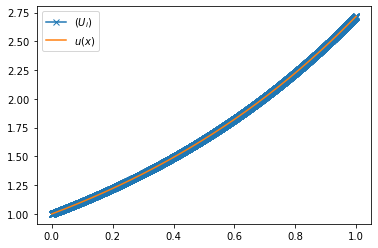
\includegraphics[width=7.5cm]{Images/preliminaires/Laplace Dirichlet 1D/solution.png}
    \caption{Graphes des solutions analytiques et approchées}
    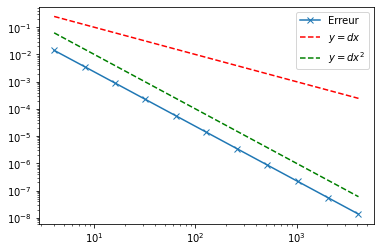
\includegraphics[width=7.5cm]{Images/preliminaires/Laplace Dirichlet 1D/analyse.png}
    \caption{Estimation de l'erreur $L^2(\Omega)$ en fonction du nombre de volumes $n$}
\end{figure}

\newpage

\section{Problème modèle en dimension deux}

De nouveau, l'analyse du problème de Poisson avec des conditions aux limites variées est traité dans \cite{brezis1983}. On a un résultat d'existence et d'unicité ainsi que l'étude de différentes régularités pour l'unique solution, cela en fonction de données variées. On trouvera aussi les résultats d'injections et de leurs propriétés des espaces Sobolev dans différents espaces fonctionnels plus classiques.

La définition d'un maillage admissible est donné chapitre 9, hypothèses 9.1 de \cite{eymard:hal-02100732} dans un contexte assez général. Nous n'utiliserons que des maillages rectangulaires, éventuellement décalés dans une ou les deux dimensions.

Ensuite vient la donnée de résultats continus connus comme l'inégalité de Poincaré, sous forme discrète pour des conditions de Dirichlet sur chaque bord. Sous réserve de connexité d'$\Omega$, il est possible de l'obtenir avec Dirichlet sur une face seulement.

La section 9.3 démontre l'existence et l'unicité d'une solution discrète pour le problème de Dirichlet par l'estimation de la norme $H^1_0(\Omega$ en fonction du diamètre de $\Omega$ et de la norme $L^2(\Omega)$ du second membre. 

Ensuite la notion de convergence est largement étudiée pour différentes régularités des données, et donc de la solution. 

\subsection*{Un exemple}

Soit $\Omega := (0,1) \times (0,1)$, ouvert connexe borné lipschtizien de $\mathbb{R}^2$. Soit $u: x, y \mapsto cos(2\pi x) sin(2\pi y)$, analytique sur $\Omega$. Cette fonction est solution du problème de Dirichlet 2.D
\begin{equation*}
\left\{\begin{array}{rll}
    \Delta u(x,y) & = -8 \pi^2 u(x, y) & \forall x,y \in \Omega \\
    u_{|\partial \Omega} & = u^D(x, y) & \forall x,y \in \partial \Omega
\end{array}
\right.
\end{equation*}

On discrétise $\Omega$ en un ensemble de $n_y \times n_x$ volumes élémentaires. On introduit les pas d'espace en chaque dimension $\Delta x := 1/n_x$ et $\Delta y := 1/n_y$. Les arêtes verticales sont de mesure uniforme $\Delta y$ et les arêtes horizontales de mesure $\Delta x$. Les centres des faces horizontales (à gauche et à droite des volumes) ont pour absisses les éléments de $\{ x_i \}_{i \in \llbracket 0, n_x \rrbracket} = \{ i \Delta x \}$ et pour ordonnées $\{ y_{j+1/2} \}_{j \in \llbracket 0, n_y-1 \rrbracket} = \{ (j+1/2) \Delta y \}_{j}$, les centres des faces verticales (au-dessus et en dessous des volumes) ont pour absisses $\{ x_{i+1/2} \}_{i \in \llbracket 0, n_x-1 \rrbracket} = \{ (i+1/2) \Delta x \}_i$ et pour ordonnées $\{ y_j \}_{j \in \llbracket 0, ny \rrbracket} = \{j \Delta y\}_j$. Enfin, les centres des volumes sont aux absisses et ordonnées d'indice semi-entières.

Les noeuds de vitesse $U_h$ sont positionnés aux centres des volumes et également sur le bord $\partial \Omega$ où ils sont donnés par les conditions de Dirichlet, c.f la figure suivante

\begin{figure}[htp]
    \centering
    \includegraphics[width=5cm]{Images/preliminaires/maillages/centré 2D.png}
    \caption{Maillage structuré uniforme de $\bar{\Omega}=[0,1]^2$ en $8 \times 8$ volumes à l'intérieur. Les points bleus à l'intérieur en sont les centres.}
\end{figure}

\newpage

Ce maillage est \textit{admissible} au sens des hypothèses 9.2 de \cite{eymard:hal-02100732}. 

On ne numérote que les inconnues à l'intérieur du domaine, les autres étant résolues ensuite, en commençant par celle située en bas à gauche et en suivant l'ordre lexicographique, du bas vers le haut. La correspondance entre l'indice $k$ de l'inconnue et son repérage $(j,i)$ sur la grille se fait par la relation $k = j(n_x+2) + i$. Réciproquement, $i = k \% (n_x+2)$, reste de la division euclidienne (écrite avec le symbole Python) et $j = k // (n_x+2)$, quotient de la division euclidienne (symbole Python).

\paragraph{Formulation du système linéaire} Le système linéaire associé au problème est donné par
\begin{equation*}
    \frac{\Delta y}{\Delta x} \left( U_{h, j, i+1} - 2 U_{h, j, i} + U_{h, j, i+1} \right) + \frac{\Delta x}{\Delta y} \left( U_{h, j+1, i} - 2 U_{h, j, i} + U_{h, j-1, i} \right) = (\Delta y \Delta x) f_{j,i}
\end{equation*}
si $U_{h, j, i}$ est à l'intérieur du domaine $\Omega$ et sans flux au bord, sans arête incluse dans $\partial \Omega$. Si $U_{h, j, i}$ est au centre d'un volume possédant une arête sur un bord, alors un des points $U_{h, j+1, i}$, $U_{h, j-1, i}$, $U_{h, j, i+1}$, $U_{h, j, i-1}$ au moins est fictif. Dans ce cas on substitue sa valeur dans le bilan de flux. 

Par exemple, si $j=0$, alors $\frac{U_{h, 0, i + U_{h, -1, i}}}{2} = u^D_{0,i}$, et on peut substituer $U_{h, -1, i}$ dans la formule précédente par une expression faisant intervenir un noeud existant et une donnée qui passe au second membre. Pour ce maillage, la technique est identique sur chaque bord. Plutôt que rallonger ce texte, passons au code et à son résultat. 

\begin{minted}{python}
from matplotlib import pyplot
import numpy

u_func = lambda x, y: numpy.cos(2*numpy.pi*x)*numpy.sin(2*numpy.pi*y)
f_func = lambda x, y: -8*numpy.pi**2 * numpy.cos(2*numpy.pi*x) * \
                       numpy.sin(2*numpy.pi * y)
x0 = 0.
x1 = 1
y0 = 0.
y1 = 1

nx_ = numpy.array([4, 8, 16, 32, 64, 128])
dx_ = numpy.empty(nx_.shape[0])
err = numpy.empty(nx_.shape[0])

for l, nx in enumerate(nx_):
    ny = nx
    dx = (x1 - x0) / nx
    dy = (y1 - y0) / ny
    dx_[l] = dx
    print("===== Simulation sur {}x{} volumes. =====".format(ny, nx))
    
    # Discrétisation spatiale
    x_f = numpy.linspace(x0, x1, nx+1)
    x_c = numpy.linspace(x0+dx/2, x1-dx/2, nx)
    x_  = numpy.concatenate([[x0], x_c, [x1]])
    
    y_f = numpy.linspace(y0, y1, ny+1)
    y_c = numpy.linspace(y0+dy/2, y1-dy/2, ny)
    y_  = numpy.concatenate([[y0], y_c, [y1]])
    
    X_c, Y_c = numpy.meshgrid(x_c, y_c)
    X_, Y_   = numpy.meshgrid(x_, y_)
    
    # Vecteur solution analytique
    u = u_func(X_, Y_)
    
    # Initialisation
    U = numpy.empty((ny+2, nx+2))
    
    indices_bords = {
            'bas': [i for i in range(nx)],
            'droit': [(j+1)*nx-1 for j in range(ny)],
            'haut': [(ny-1)*nx+i for i in range(nx)],
            'gauche': [j*nx for j in range(ny)]
        }
    
    # Système linéaire
    b = (dx*dy) * f_func(X_c, Y_c)
    b = b.flatten()
    
    A = -2 * (dy/dx + dx/dy) * numpy.eye(nx*ny) + \
        dy/dx * numpy.diag(numpy.ones(nx*ny-1), 1) + \
        dy/dx * numpy.diag(numpy.ones(nx*ny-1),-1) + \
        dx/dy * numpy.diag(numpy.ones(nx*ny-nx), nx) + \
        dx/dy * numpy.diag(numpy.ones(nx*ny-nx),-nx)
        
    # Modifications des noeuds ayant un flux au bord
    for k in indices_bords['bas']:
        A[k, k] -= dx/dy
        b[k] -= 2 * dx/dy * u_func(x_c[k%nx], y0)
    for k in indices_bords['droit']:
        if k < nx*ny-1: A[k, k+1] = 0
        A[k, k] -= dy/dx
        b[k] -= 2 * dy/dx * u_func(x1, y_c[k//nx])
    for k in indices_bords['haut']:
        A[k, k] -= dx/dy
        b[k] -= 2 * dx/dy * u_func(x_c[k%nx], y0)
    for k in indices_bords['gauche']:
        if k > 1: A[k, k-1] = 0
        A[k, k] -= dy/dx
        b[k] -= 2 * dy/dx * u_func(x0, y_c[k//nx])
        
    U[1:-1, 1:-1] = numpy.linalg.solve(A, b).reshape((ny, nx))
    U[0, :] = u_func(x_, y0)
    U[-1,:] = u_func(x_, y1)
    U[:, 0] = u_func(x0, y_)
    U[:,-1] = u_func(x1, y_)
    
    err[l] = numpy.sqrt(dy*dx) * numpy.linalg.norm(U-u, ord=2)

pyplot.imshow(numpy.abs(U-u))
pyplot.colorbar()
pyplot.show()

pyplot.loglog(nx_, dx_, 'r--', label=r"$\Delta x$")
pyplot.loglog(nx_, dx_**2, 'b--', label=r"$\Delta x^2$")
pyplot.loglog(nx_, err, label='x', marker="x")
pyplot.legend()
pyplot.show()
\end{minted}
Qui rend les figures
\begin{figure}[htp]
    \centering
    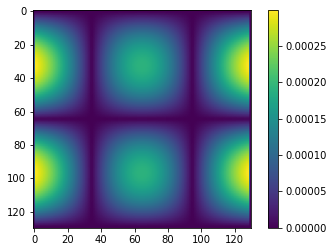
\includegraphics[width=7.5cm]{Images/preliminaires/Laplace Dirichlet 2D/erreur.png}
    \caption{Champ d'erreurs $| U_h - u_h |$ pour $n=128^2$ volumes}
    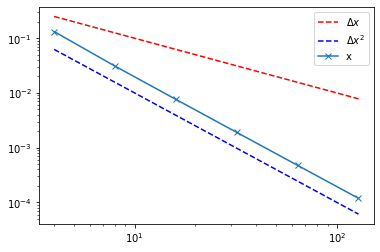
\includegraphics[width=7.5cm]{Images/preliminaires/Laplace Dirichlet 2D/analyse.png}
    \caption{Estimation de l'erreur $L^2(\Omega)$ en fonction du nombre de volumes $n$}
    \label{fig:laplacienDirichlet1D}
\end{figure}

\newpage

Bien que le graphe soit satisfaisant, nous faisons face ici à deux problèmes majeurs : le temps de calcul ainsi que la complexité mémoire de l'algorithme. Le temps de calcul pour ce programme est d'en moyenne 44.8s avec un écart de type de 13s, comme on le voit sur la figure \ref{fig:laplacienDirichlet2Dtemps}
\begin{figure}[htp]
    \centering
    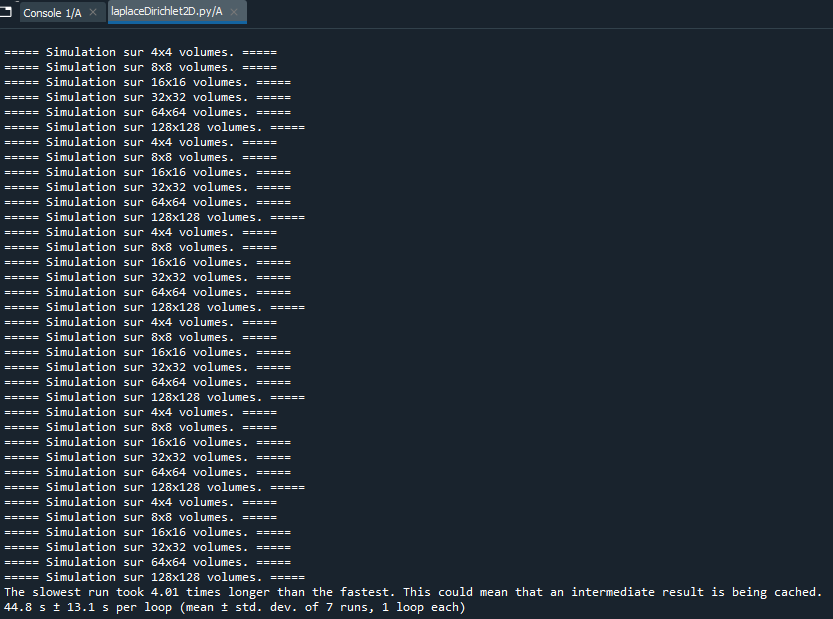
\includegraphics[width=7.5cm]{Images/preliminaires/Laplace Dirichlet 2D/temps.png}
    \caption{Sortie console de la commande \textit{magic} \textbf{\%timeit} de l'enironnement interactif de Python : sur 7 essais, il rend la durée moyenne de l'exécution et son l'écart-type.}
    \label{fig:laplacienDirichlet2Dtemps}
\end{figure}

D'autre part, si cette exécution est effectuée sur une grille carrée de taille $128 \times 128$, le passage à $256 \times 256$ n'est plus possible sur un ordinateur personnel. En effet, l'implémentation du système linéaire en tant qu'objet plein demande dans ce cas $32$ GiB de données pour stocker la matrice du système linéaire dans le format \textit{float64}. On peut le vérifier sur la figure \ref{fig:laplacienDirichlet2Dmemoire}
\begin{figure}[htp]
    \centering
    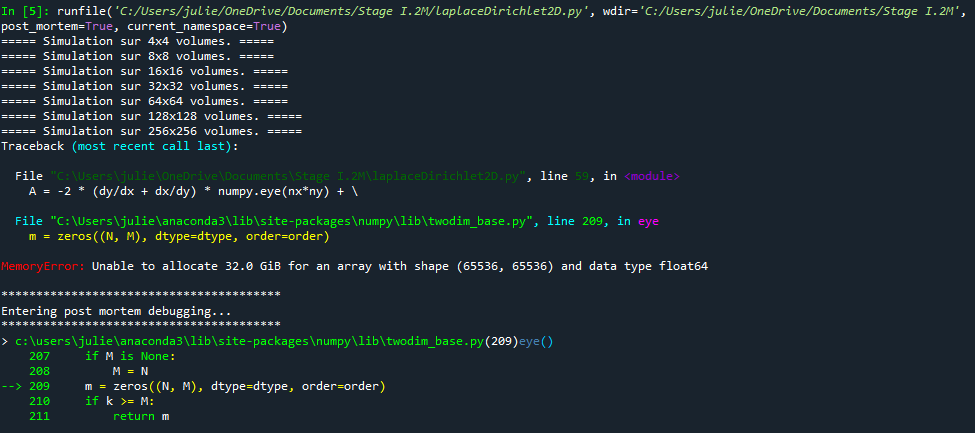
\includegraphics[width=7.5cm]{Images/preliminaires/Laplace Dirichlet 2D/memoire.png}
    \caption{Erreur rendue lors de l'exécution de la simulation pour $256 \times 256$ volumes.}
    \label{fig:laplacienDirichlet2Dmemoire}
\end{figure}

\newpage

Afin de palier à ces problèmes, on retente l'expérience avec l'implémentation en matrices creuses. Ces objets sont implémentés dans la bibliothèque \textbf{Scipy}, plus précisément dans la sous-librairie \textbf{Scipy.sparse}. Une matrice creuse est une manière de représenter les matrices en ne gardant en mémoire que ses entrées non-nulles. Pour l'implémenter, on prescrit trois tableaux, contenant la ligne de la donnée à stocker, la ligne puis la colonne où elle se trouve. Par exemple, la représentation creuse de $$ \begin{pmatrix} 9 & 0 & 0 & 0 & 0 \\ 0 & 0 & 8 & 0 & 0 \\ 0 & 7 & 0 & 0 & 0 \\ 0 & 0 & 0 & 0 & 0 \\ 0 & 0 & 0 & 6 & 5 \end{pmatrix} $$ est donnée par le triplet \begin{center}
\begin{tabular}{ |l||c|c|c|c|c| } 
\hline
donnée & 9 & 8 & 7 & 6 & 5 \\ 
\hline
ligne & 1 & 2 & 3 & 5 & 5 \\ 
\hline
colonne & 1 & 3 & 2 & 4 & 5 \\ 
\hline
\end{tabular}
\end{center}

\subsection*{Laplacien de Dirichlet 2.D revisité} 

On reprend un problème de Dirichlet en deux dimensions d'espace avec maintenant la déclaration de l'opérateur laplacien en matrices creuses. Cette fois, on considère les noeuds de l'inconnue discrète $U_h$ sur les faces des volumes élémentaires et on les comptes dans le système

\begin{figure}[htp]
    \centering
    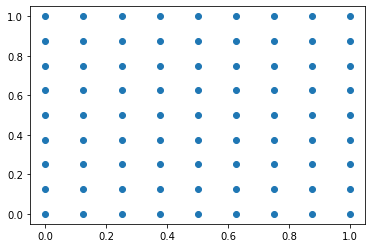
\includegraphics[width=7.5cm]{Images/preliminaires/maillages/bords 2D.png}
    \caption{Localisation des noeuds en lesquels est définie $U_h$}
\end{figure}

On vérifie que ce changement de convention n'a aucune incidence notable sur la résolution du problème.

\begin{minted}{python}
from matplotlib import pyplot
import numpy
from numpy import cos, pi, sin
import scipy
from scipy import sparse
from scipy.sparse import linalg

# SETUP
u_func  = lambda x, y : sin(x)*cos(y)
f_func = lambda x, y : 2 * u_func(x, y)

# DISCRETISATION SPATIALE
## horizontale
xi = 0.
xf = 2*pi
L  = (xf-xi)
nx_ = numpy.array([4, 8, 16, 32, 64, 128, 256, 512, 1024])
dx_ = L/nx_
## verticale
yi = 0.
yf = 2*pi
H  = (yf-yi)

# INITIALISATION DES ERREURS
err = numpy.zeros(nx_.shape)

# ITERATION SPATIALE
for l, nx in enumerate(nx_):
    
    dx = dx_[l]
    # DISCRETISATION SPATIALE CARREE
    ny = nx
    dy = H/ny
    ## Info
    print("> Simulation sur maillage {}x{}".format(ny, nx))
    
    # CONSTRUCTION DE LA GRILLE 
    x_  = numpy.linspace(xi, xf, nx+1)
    y_  = numpy.linspace(yi, yf, ny+1)
    x_u, y_u = numpy.meshgrid(x_, y_)
     
    # DECLARATION DE L'OPERATEUR (-) LAPLACIEN DE DIRICHLET DISCRET CREUX
    n = 5 * (ny-1)*(nx-1) + 2*nx + 2*ny
    
    lignes   = numpy.zeros(n)
    colonnes = numpy.zeros(n)
    donnees  = numpy.zeros(n)
    compteur = 0
    
    b = dy*dx * f_func(x_u, y_u)
    b[0, :] = u_func(x_, yi)
    b[-1,:] = u_func(x_, yf)
    b[:, 0] = u_func(xi, y_)
    b[:,-1] = u_func(xf, y_)
    
    for j in range(ny+1):
        for i  in range(nx+1):
            
            if i == 0 or i == nx or j == 0 or j == ny:
                lignes[compteur]   = j * (nx+1) + i
                colonnes[compteur] = j * (nx+1) + i
                donnees[compteur]  = 1
                compteur += 1
            
            else:
                lignes[compteur:compteur+5] = j * (nx+1) + i
                colonnes[compteur]   = j * (nx+1) + i
                colonnes[compteur+1] = j * (nx+1) + i - 1
                colonnes[compteur+2] = j * (nx+1) + i + 1
                colonnes[compteur+3] = (j-1) * (nx+1) + i
                colonnes[compteur+4] = (j+1) * (nx+1) + i
                donnees[compteur]   = 2 * (dy/dx + dx/dy)
                donnees[compteur+1] = -dy/dx
                donnees[compteur+2] = -dy/dx
                donnees[compteur+3] = -dx/dy
                donnees[compteur+4] = -dx/dy
                compteur += 5
    
    A = sparse.coo_matrix((donnees, (lignes, colonnes)), shape=((ny+1)*(nx+1), (ny+1)*(nx+1))).tocsr()
    
    # RESOLUTION
    U = linalg.spsolve(A, b.flatten()).reshape((ny+1, nx+1))
    
    # ANALYSE
    u = u_func(x_u, y_u)
    err[l] = numpy.sqrt(dy*dx) * numpy.linalg.norm(U-u, ord=2)
    
# FIGURES
pyplot.figure()
pyplot.loglog(nx_, err, 'x-', label=r"$||U-u||_{L^2}$")
pyplot.loglog(nx_, dx_, '--', label=r"$\Delta x$")
pyplot.loglog(nx_, dx_**2, '--', label=r"$\Delta x^2$")
pyplot.legend()
pyplot.show()

pyplot.figure()
pyplot.imshow(numpy.abs(U-u))
pyplot.colorbar()
pyplot.show()
\end{minted}
On trouve les courbes
\begin{figure}[htp]
    \centering
    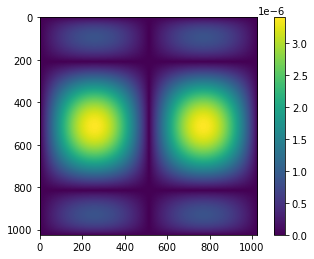
\includegraphics[width=7cm]{Images/preliminaires/Laplace Dirichlet 2D creux/erreur.png}
    \caption{Erreur rendue lors de l'exécution de la simulation pour $1024 \times 1024$ volumes.}
    \label{fig:creuxLaplacien2DErreur}
\end{figure}
\begin{figure}[htp]
    \centering
    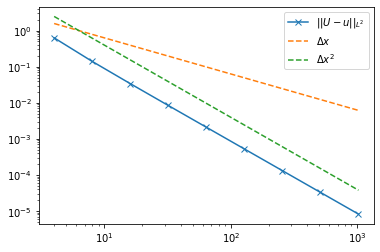
\includegraphics[width=7cm]{Images/preliminaires/Laplace Dirichlet 2D creux/analyse.png}
    \caption{Estimation de l'erreur $L^2(\Omega)$ pour des maillages entre $4 \times 4$ et $1024 \times 1024$ volumes.}
    \label{fig:creuxLaplacien2DAnalyse}
\end{figure}
\begin{figure}[htp]
\centering
    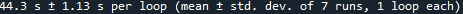
\includegraphics[width=10cm]{Images/preliminaires/Laplace Dirichlet 2D creux/temps.png}
    \caption{Estimation de la durée de l'exécution pour $1024 \times 1024$ volumes.}
    \label{fig:creuxLaplacienDirichlet2DTemps}
\end{figure}

Afin de pouvoir comparer aisément les temps d'exécutions avec d'autres méthodes, on redonne l'analyse temporelle pour l'analyse du schéma entre $4$ et $512$ volumes par dimension. On trouve plutôt

\begin{figure}[!htp]
\centering
    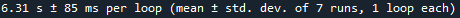
\includegraphics[width=10cm]{Images/preliminaires/Laplace Dirichlet 2D creux/temps2.png}
    \caption{Estimation de la durée de l'exécution pour $512 \times 512$ volumes.}
    \label{fig:creuxLaplacienDirichlet2DTemps2}
\end{figure}

\newpage

\section{Résolution par méthode G.M.R.E.S}

\subsection*{Expérience numérique} 

On reprend exactement la simulation de la partie précédente, avec au maximum $512$ volumes par dimension, en substituant à
\begin{minted}{python}
    U = linalg.spsolve(A, b.flatten()).reshape((ny+1, nx+1))
\end{minted}
la ligne
\begin{minted}{python}
    U = linalg.gmres(A, b.flatten())[0].reshape((ny+1, nx+1))
\end{minted}
et on reproduit l'estimation de la durée. On trouve, pour cette méthode de résolution, les graphes suivants
\begin{figure}[!htp]
    \centering
    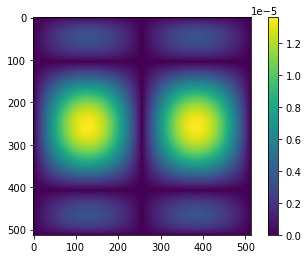
\includegraphics[width=7cm]{Images/preliminaires/Laplace Dirichlet 2D creux GMRES/erreur.png}
    \caption{Erreur rendue lors de l'exécution de la simulation pour $512 \times 512$ volumes.}
    \label{fig:creuxLaplacien2DGMRESErreur}
\end{figure}

\begin{figure}[htp]
\centering
    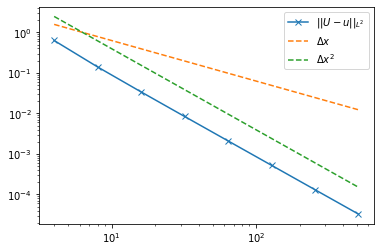
\includegraphics[width=7cm]{Images/preliminaires/Laplace Dirichlet 2D creux GMRES/analyse.png}
    \caption{Estimation de l'erreur $L^2(\Omega)$ pour des maillages entre $4\times 4$ et $512 \times 512$ volumes.}
    \vspace{1cm}
    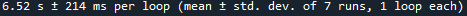
\includegraphics[width=10cm]{Images/preliminaires/Laplace Dirichlet 2D creux GMRES/temps.png}
    \caption{Compte-rendu de l'estimation de la durée de l'exécution de l'analyse jusqu'à $512 \times 512$ volumes.}
    \label{fig:creuxLaplacienDirichlet2DGMRESTemps}
\end{figure}

\newpage

En guise de commentaire, on remarque que la convergence est bien assurée mais le gain de temps est très incertain, en fait le temps moyen est même supérieur à celui affiché par la méthode directe. L'appel à la méthode G.M.R.E.S n'est donc ici d'aucune utilité.

\section{Résolution par la méthode BI.C.G.STAB}

\subsection*{Expérience numérique} 

Une dernière fois on essaie de résoudre le système linéaire modèle à l'aide de cette nouvelle méthode. La résolution se fait en substituant à la ligne
\begin{minted}{python}
    U = linalg.spsolve(A, b.flatten()).reshape((ny+1, nx+1))
\end{minted}
la ligne
\begin{minted}{python}
    U = linalg.bicgstab(A, b.flatten())[0].reshape((ny+1, nx+1))
\end{minted}
L'estimation du temps d'exécution rend
\begin{figure}[htp]
    \centering
    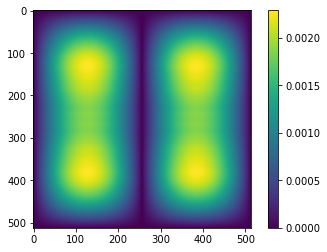
\includegraphics[width=7cm]{Images/preliminaires/Laplace Dirichlet 2D creux BICGSTAB/erreur.png}
    \caption{Erreur rendue lors de l'exécution de la simulation pour $512 \times 512$ volumes.}
    \label{fig:creuxLaplacien2DBICGSTABErreur}
\end{figure}

\begin{figure}[htp]
    \centering
    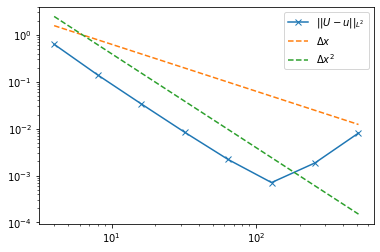
\includegraphics[width=7cm]{Images/preliminaires/Laplace Dirichlet 2D creux BICGSTAB/analyse.png}
    \caption{Estimation de l'erreur $L^2(\Omega)$ pour des maillages entre $4\times 4$ et $512 \times 512$ volumes.}
    \label{fig:creuxLaplacien2DBICGSTABAnalyse}
\end{figure}

\begin{figure}[htp]
\centering
    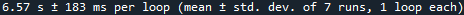
\includegraphics[width=10cm]{Images/preliminaires/Laplace Dirichlet 2D creux BICGSTAB/temps.png}
    \caption{Compte-rendu de l'estimation de la durée de l'exécution de l'analyse jusqu'à $512 \times 512$ volumes.}
    \label{fig:creuxLaplacienDirichlet2DBICGSTABTemps}
\end{figure}

\newpage

Cette fois, le problème est plus grave : la méthode diverge pour les trois maillages les plus fins. Si le temps d'exécution est sensiblement équivalent aux deux premières méthodes, directes et GMRES, la méthode BICGSTAB se comporte en fait mal vis-à-vis de l'opérateur implémenté.

\section{Conclusion de la comparaison des méthodes}

Il existe une faille dans ce qui précède. Elle est de l'ordre de l'implémentation, mes tests ne portaient pas uniquement sur la résolution du système linéaire mais également sur l'affichage de l'information de l'avancement de l'algorithme et sur l'affichage des courbes. Ces deux opérations peuvent être pénalisantes selon le langage utilisé et viennent biaiser cette analyse. La même analyse effectuée en supprimant les éléments d'affichage et de calcul d'erreur (on ne conserve que l'assemblage et la résolution de l'équation, pour chaque maillage entre $4 \times 4$ ... $512 \times 512$, on obtient à nouveau des temps sensiblement équivalents pour la méthode directe et la méthode BICGSTAB, en revanche je ne m'explique pas le bond de durée de la simulation pour la méthode GMRES. On reproduit encore les estimations
\begin{figure}[htp]
\centering
    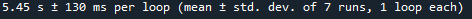
\includegraphics[width=12cm]{Images/preliminaires/Laplace Dirichlet 2D creux/temps3.png}
    \caption{Compte-rendu de l'estimation de la durée de l'exécution de l'analyse jusqu'à $512 \times 512$ volumes par méthode directe.}
    
    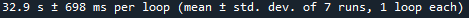
\includegraphics[width=12cm]{Images/preliminaires/Laplace Dirichlet 2D creux GMRES/temps2.png}
    \caption{Compte-rendu de l'estimation de la durée de l'exécution de l'analyse jusqu'à $512 \times 512$ volumes par méthode GMRES.}
    
    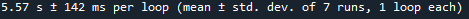
\includegraphics[width=12cm]{Images/preliminaires/Laplace Dirichlet 2D creux BICGSTAB/temps2.png}
    \caption{Compte-rendu de l'estimation de la durée de l'exécution de l'analyse jusqu'à $512 \times 512$ volumes par méthode BICGSTAB.}
    \label{fig:creuxLaplacienDirichlet2DConclusion}
\end{figure}

\section{La question du préconditionnement}

De même que les méthodes itératives sont supposées accélérer la convergence des solutions approchées, il est possible de faire un pas supplémentaire dans l'accélération à l'aide des méthodes de l'usage de préconditionnement. Dans cette partie, on reprend l'étude du problème modèle en implémentant un des deux préconditionnements : factorisation \textbf{LU}, factorisation \textbf{ILU}, ou LU incomplète.

\subsection*{Expérience numérique avec factorisation LU}

Le préconditionnement L.U pour les matrices creuses peut s'obtenir, en langage Python, grâce à la classe \textbf{LinearOperator} de la sous-librairie \textbf{scipy.sparse.linalg}. Une fois l'opérateur creux déclaré, il suffit de continuer par les deux lignes
\begin{minted}{python}
Alu  = scipy.sparse.linalg.splu(A) # Objet contenant une méthode .solve() qui est le préconditionneur
Apre = scipy.sparse.linalg.LinearOperator( ((ny+1)*(nx+1), (ny+1)*(nx+1)), Alu.solve )
\end{minted}
et la dernière variable est à passer en argument de la fonction de résolution du système
\begin{minted}{python}
U = scipy.sparse.linalg.gmres(A, b.flatten(), M=Apre)[0].reshape((ny+1, nx+1))
\end{minted}
ou
\begin{minted}{python}
U = scipy.sparse.linalg.bicgstab(A, b.flatten(), M=Apre)[0].reshape((ny+1, nx+1))
\end{minted}
L'estimation du temps moyen de l'analyse pour le problème de Dirichlet 2.D devient alors, respectivement
\begin{figure}[htp]
\centering
    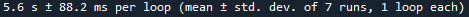
\includegraphics[width=12cm]{Images/preliminaires/Laplace Dirichlet 2D creux GMRES Precond/tempsLU.png}
    \caption{Estimation de la durée de l'exécution de l'analyse jusqu'à $512 \times 512$ volumes par méthode GMRES et préconditionnement LU.}
    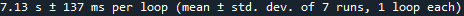
\includegraphics[width=12cm]{Images/preliminaires/Laplace Dirichlet 2D creux BICGSTAB Precond/tempsLU.png}
    \caption{Estimation de la durée de l'exécution de l'analyse jusqu'à $512 \times 512$ volumes par méthode BICGSTAB et préconditionnement LU.}
    \label{fig:preconditionnementLU}
\end{figure}

On constate un léger avantage de la méthode GMRES pour ce préconditionnement quant à la vitesse d'exécution, mais qu'en est-il des erreurs pour ces deux méthodes ? On donne les couples champ d'erreur et analyse d'abord pour GMRES puis pour BICGSTAB ci-après.

\begin{figure}[htp]
    \centering
    \includegraphics[width=7cm]{Images/preliminaires/Laplace Dirichlet 2D creux GMRES Precond/erreurLU.png}
    \caption{Erreur rendue lors de l'exécution de la simulation pour $512 \times 512$ volumes avec GMRES / LU.}
\end{figure}

\begin{figure}[htp]
    \centering
    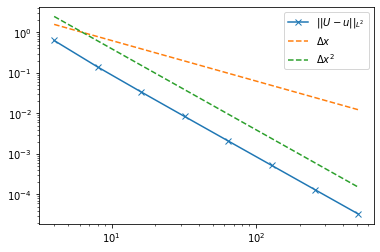
\includegraphics[width=7cm]{Images/preliminaires/Laplace Dirichlet 2D creux GMRES Precond/analyseLU.png}
    \caption{Analyse rendue lors de l'exécution de la simulation pour $512 \times 512$ volumes avec GMRES / LU.}
    \label{fig:creuxLaplacien2DGMRESPrecondLU}
\end{figure}

\begin{figure}[htp]
    \centering
    \includegraphics[width=7cm]{Images/preliminaires/Laplace Dirichlet 2D creux BICGSTAB Precond/erreurLU.png}
    \caption{Erreur rendue lors de l'exécution de la simulation pour $512 \times 512$ volumes avec BICGSTAB / LU.}
\end{figure}

\begin{figure}[htp]
    \centering
    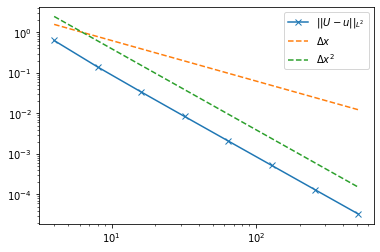
\includegraphics[width=7cm]{Images/preliminaires/Laplace Dirichlet 2D creux GMRES Precond/analyseLU.png}
    \caption{Analyse rendue lors de l'exécution de la simulation pour $512 \times 512$ volumes avec BICGSTAB / LU.}
    \label{fig:creuxLaplacien2DBICGSTABPrecondLU}
\end{figure}

En conclusion, les deux méthodes appelées avec un préconditionnement LU donnent des erreurs $L^2(\Omega)$ sensiblement équivalentes. On constate la convergence à l'ordre 2 en espace et BICGSTAB se montre un rien plus rapide.

\newpage 

\subsection*{Expérience numérique avec factorisation ILU}

Toujours selon le même protocole, on étudie d'abord l'efficacité de la résolution du système linéaire seul puis dans un second temps on étudie les champs d'erreurs ainsi que l'analyse de la convergence en espace pour chacune des deux méthodes.

\begin{figure}[htp]
    \centering
    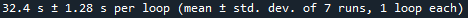
\includegraphics[width=12cm]{Images/preliminaires/Laplace Dirichlet 2D creux GMRES Precond/tempsILU.png}
    \caption{Estimation de la durée de l'exécution de l'analyse jusqu'à $512 \times 512$ volumes par méthode GMRES et préconditionnement ILU.}
\end{figure}

\begin{figure}[htp]
    \centering
    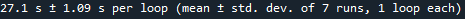
\includegraphics[width=12cm]{Images/preliminaires/Laplace Dirichlet 2D creux BICGSTAB Precond/tempsILU.png}
    \caption{Estimation de la durée de l'exécution de l'analyse jusqu'à $512 \times 512$ volumes par méthode BICGSTAB et préconditionnement ILU.}
\end{figure}
A nouveau, BICGSTAB se montre meilleur sur la vitesse d'exécution que GMRES. Vient le moment de vérifier les convergences spatiales.

\begin{figure}[htp]
    \centering
    \includegraphics[width=7cm]{Images/preliminaires/Laplace Dirichlet 2D creux GMRES Precond/erreurLU.png}
    \caption{Erreur rendue lors de l'exécution de la simulation pour $512 \times 512$ volumes avec GMRES / ILU.}
\end{figure}

\begin{figure}[htp]
    \centering
    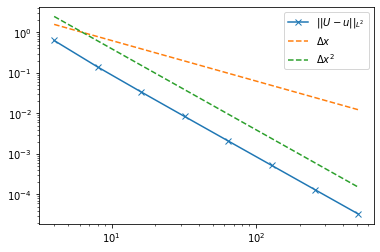
\includegraphics[width=7cm]{Images/preliminaires/Laplace Dirichlet 2D creux GMRES Precond/analyseLU.png}
    \caption{Analyse rendue lors de l'exécution de la simulation pour $512 \times 512$ volumes avec GMRES / ILU.}
    \label{fig:creuxLaplacien2DGMRESPrecondILU}
\end{figure}

\begin{figure}[htp]
    \centering
    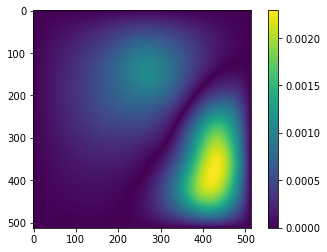
\includegraphics[width=7cm]{Images/preliminaires/Laplace Dirichlet 2D creux BICGSTAB Precond/erreurILU.png}
    \caption{Erreur rendue lors de l'exécution de la simulation pour $512 \times 512$ volumes avec BICGSTAB / ILU.}
\end{figure}

\begin{figure}[htp]
    \centering
    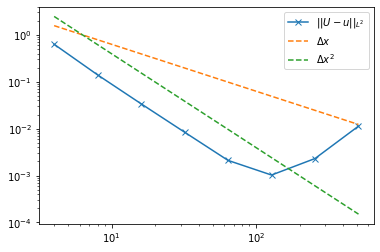
\includegraphics[width=7cm]{Images/preliminaires/Laplace Dirichlet 2D creux GMRES Precond/analyseILU.png}
    \caption{Analyse rendue lors de l'exécution de la simulation pour $512 \times 512$ volumes avec BICGSTAB / ILU.}
    \label{fig:creuxLaplacien2DBICGSTABPrecondILU}
\end{figure}

\newpage

Pour une raison que j'ignore, si GMRES parvient parfaitement à obtenir l'ordre 2 en espace attendu, BICGSTAB est mis en échec sur les deux maillages les plus fins. Ainsi, bien qu'il s'exécute plus rapidement que son concurrent GMRES / ILU, le couple BICGSTAB / ILU ne peut convenir pour notre étude.

\section{Conclusion}

Ainsi s'achève le premièr chapitre de ce mémoire, consacré au choix des outils permettant ensuite d'attaquer les études numériques à suivre. Notre choix se portera donc sur le couple GMRES/LU pour la résolution des systèmes linéaires à venir, lesquels seront représentés par des objets creux, pour des raisons de complexité mémoire.

Bien sûr, cette étude est loin d'être complète : on devrait discuter le choix des "métriques" utilisées pour effectuer ce choix. N'a-t-on pas accès au nombre d'itérations plutôt qu'à une commande boîte noire offerte par IPython, grandeur plus objective caractérisant la performance de l'algorithme ? Nous n'avons pas validé le fait que le temps compté est uniquement le temps de résolution et non celui, pourquoi pas prépondérant, d'un appel quelconque n'ayant rien à voir avec les méthodes en elles-même ? Je ne suis pas assez familier de Python pour répondre à toutes ces questions et je présente cela plus comme un exercice de style consistant à montrer qu'il faut y penser que comme une étude aboutie démontrant définitivement que le bon choix est celui annoncé.